\documentclass{beamer}

\mode<presentation>{
\usetheme{Madrid}
%\usecolortheme{beaver}
}
\usepackage[utf8]{inputenc}
%\usepackage{default}
%\usepackage[portuguese]{babel}
%\usepackage{pgfplots}
%\pgfplotsset{/pgf/number format/use comma,compat=newest}
%\usepackage{color}
\usepackage{amsfonts}
\usepackage{mathrsfs}  

%\usepackage{hyperref}


%MEUS COMANDOs

\usepackage{tikz}
\usetikzlibrary{quotes, angles, intersections}
\newcommand{\R}{\mathbb{R}}
\newcommand{\D}{\mathscr{D}}
\newcommand{\Pp}{\mathscr{P}}
\newcommand{\Cc}{\mathscr{C}}
\newcommand{\E}{\mathscr{E}}

\newcommand{\bigO}{\mathscr{O}}

\usepackage{pgfplots}
\pgfplotsset{compat=1.4}
\usepackage{algorithmicx}
\usepackage{algorithm}
%\usepgfplotslibrary{external}
%\tikzexternalize



%FIM MEUS COMANDOS

\title[Qualificação de Mestrado]{Planar Maximal Covering with Ellipses}
\author[Tedeschi, D. F.]{Danilo F. Tedeschi}
\institute[ICMC]{Instituto de Ciências Matemáticas e Computação}
\date{\today}

\begin{document}

\begin{frame}
 \maketitle
\end{frame}

\begin{frame}
\frametitle{Contents}
 \tableofcontents
\end{frame}

\section{Introduction}
\begin{frame}
\frametitle{Introduction}
\begin{itemize}
	\item Covering problems
	\begin{itemize}
		\item Set Cover Problem
		\item Maximal Covering Problem
	\end{itemize}
	\item Maximal Covering Location Problem (MCLP)
	\item Planar Maximal Covering Location Problem (PMCLP)
	\begin{itemize}
	\item One disk: $\bigO(n^2)$ and $\bigO(n^2\log{n})$ algorithms
	\item $m$ disks: $\bigO(n^{2m-1}\log{n})$ algorithm
	\end{itemize}
	\item Goals
	\begin{itemize}
		\item Develop a $\bigO(n^2\log{n})$ algorithm for the one disk case
		\item Adapt it for the $m$ ellipses case
	\end{itemize}
\end{itemize}

\end{frame} 


\section{Preliminaries}

\begin{frame}{Preliminaries}
	
	\begin{block}{Norms}
		Let $u \in \R^2$ and $Q$ a $2x2$ positive definite matrix
		\begin{itemize}
			\item Euclidean
			\begin{equation*}
			||u||_2 = \sqrt{u^Tu}
			\end{equation*}
			
			\item Elliptical
			\begin{equation*}
			||u||_{Q} = \sqrt{u^TQu}
			\end{equation*}
		\end{itemize}
	\end{block}

\end{frame}

\begin{frame}{Preliminaries}
	\begin{figure}[H]
		\centering
		
		\caption{The elliptical and euclidean norms.}
		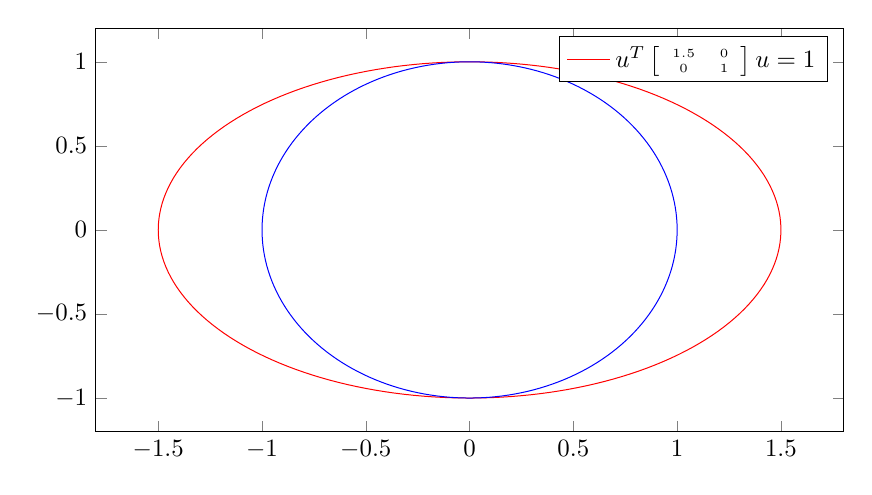
\begin{tikzpicture}[scale=0.9]
\begin{axis}[
    %axis lines = left,
    xlabel = ,
    ylabel = ,
    width=\textwidth,
    height=\axisdefaultheight
]

%Below the red parabola is defined
\addplot [domain=-pi:pi,samples=200,red]({1.5*cos(deg(x))}, {1*sin(deg(x))});

\addlegendentry{$\tiny u^T\left[\begin{array}{cc}
		1.5 & 0\\
		0 & 1
	\end{array}\right]u = 1$}
\addplot [domain=-pi:pi,samples=200,blue]({sin(deg(x))}, {cos(deg(x))});
\end{axis}
\end{tikzpicture}
		%\fautor
		\label{fig:3ellipses_intersect}
	\end{figure}
\end{frame}

\begin{frame}{Preliminaries}
	
	\begin{block}{Ellipse}
		Given a center $c \in \R^2$ and a $2x2$ p.d. matrix $Q$, an ellipse is the set of points that satisfy
		
		\begin{equation*}
		||u-c||_Q = 1,
		\end{equation*}
		
		with $\le$ representing the set of covered points
	\end{block}

	\begin{block}{Axis-parallel ellipse}
		Any $2$ by $2$ diagonal d.p. matrix determines an axis-parallel ellipse, which can also be described by
		
		\begin{equation*}
		\frac{(x-c_x)^2}{a^2} + \frac{(y-c_y)^2}{b^2} = 1,
		\end{equation*}
		
		where $(a,b)$ are the shape parameters and $c=(c_x,c_y)$ is the center.
	\end{block}

\end{frame}



\section{Maximal Covering by Disks}
\begin{frame}{Maximal Covering by Disks}{One disk}
	
	$MCD(\Pp, 1)$ is the problem of placing one disk on the plane to cover a subset of a demand set $\Pp$ maximizing the weights of the covered points.
	
	\begin{equation*}\label{eq:max_one_disk}
		\max_q w(\Pp \cap D(q)),
	\end{equation*}
	
	\begin{itemize}
		\item $\Pp=\{p_1,\dots,p_n\}$ is the demand set with weights $w(p_i)>0$
		\item $w(A)$, $A\subset \Pp$, is the sum of weights of the points in $A$
		\item $D(q)$ is a unit disk with center at point $q$
		\item \cite{chazelle:1986} proposed a $\bigO(n^2)$ algorithm
		\item \cite{drezner} proposed a $\bigO(n^2\log{n})$ which our work is based on
		\item We will introduce an equivalent problem...
	\end{itemize}
\end{frame}

\subsection{Maximum Weight Clique Problem}
\begin{frame}{Maximum Weight Clique Problem}
	Let $\D=\{D_1,\dots,D_n\}$ be a set of $n$ unit disks with weights $w_i>0$. The maximum weight clique is defined as
	
	\begin{equation*}
	\max_q \sum_{D_k \cap q \neq \emptyset} w_k,
	\end{equation*}
	
	\begin{itemize}
		\item The disks are fixed with centers at $\Pp =\{p_1,\dots,p_n\}$ with $w_k=w(p_k)$
		\item A clique is a non-empty intersection area of a subset of disks. We search for only a point in an optimal clique.
		\item An optimal solution for the maximum weight clique is an optimal solution for $MCD(\Pp,1)$.
	\end{itemize}
\end{frame}

\begin{frame}{Maximum Weight Clique Problem}{Equivalence}
		\begin{figure}[H]
		\centering
		
		\caption{An instance of $MCD(\Pp,1)$.}
		%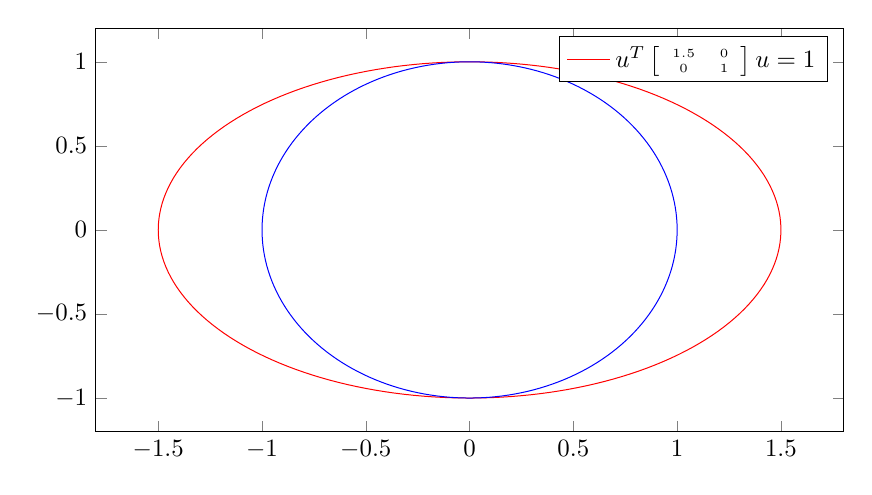
\begin{tikzpicture}[scale=0.9]
\begin{axis}[
    %axis lines = left,
    xlabel = ,
    ylabel = ,
    width=\textwidth,
    height=\axisdefaultheight
]

%Below the red parabola is defined
\addplot [domain=-pi:pi,samples=200,red]({1.5*cos(deg(x))}, {1*sin(deg(x))});

\addlegendentry{$\tiny u^T\left[\begin{array}{cc}
		1.5 & 0\\
		0 & 1
	\end{array}\right]u = 1$}
\addplot [domain=-pi:pi,samples=200,blue]({sin(deg(x))}, {cos(deg(x))});
\end{axis}
\end{tikzpicture}
      \center{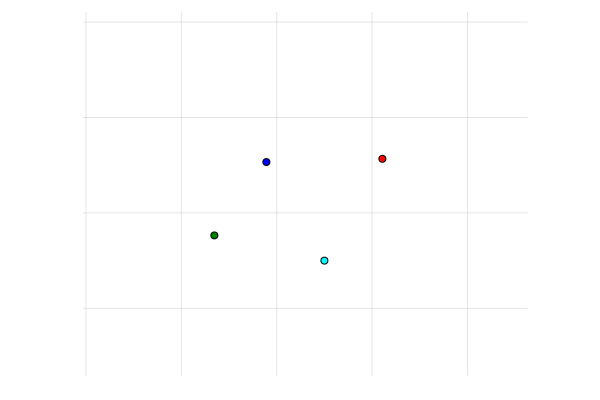
\includegraphics[width=.7\textwidth]{figures/mcd_instance.png}}
		%\fautor
		\label{fig:mcd_instance}
	\end{figure}
\end{frame}

\begin{frame}{Maximum Weight Clique Problem}{Equivalence}
	\begin{figure}[H]
		\centering
		
		\caption{An instance of Maximum Weight Clique Problem.}
		%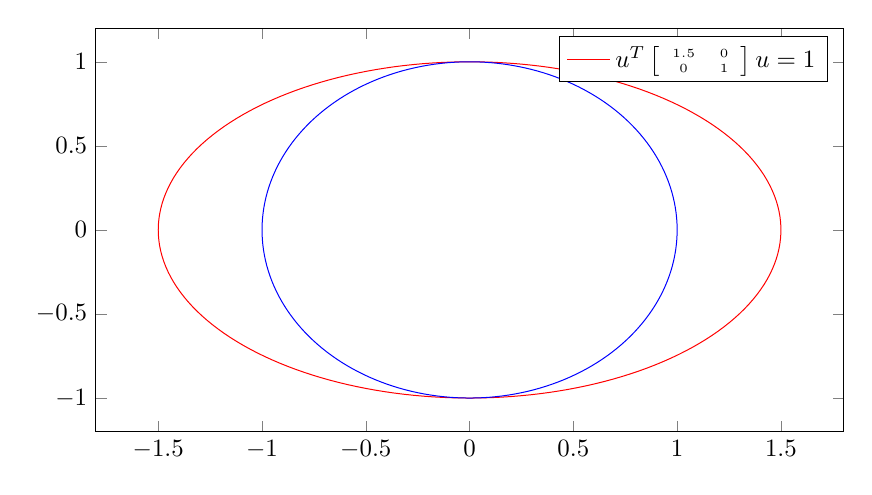
\begin{tikzpicture}[scale=0.9]
\begin{axis}[
    %axis lines = left,
    xlabel = ,
    ylabel = ,
    width=\textwidth,
    height=\axisdefaultheight
]

%Below the red parabola is defined
\addplot [domain=-pi:pi,samples=200,red]({1.5*cos(deg(x))}, {1*sin(deg(x))});

\addlegendentry{$\tiny u^T\left[\begin{array}{cc}
		1.5 & 0\\
		0 & 1
	\end{array}\right]u = 1$}
\addplot [domain=-pi:pi,samples=200,blue]({sin(deg(x))}, {cos(deg(x))});
\end{axis}
\end{tikzpicture}
		\center{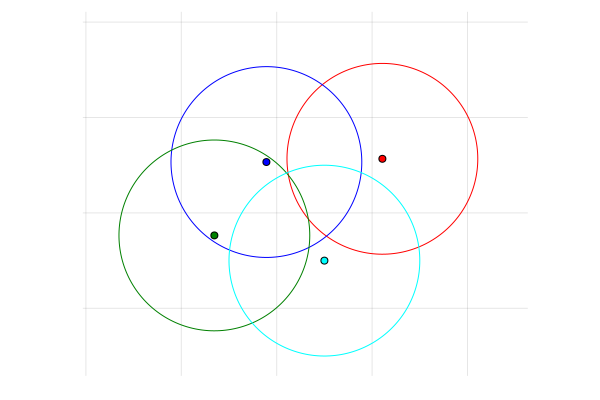
\includegraphics[width=.7\textwidth]{figures/mwc_instance.png}}
		%\fautor
		\label{fig:max_wieght_clique}
	\end{figure}
\end{frame}

\begin{frame}{Maximum Weight Clique Problem}{Algorithm}
	Let $\Gamma_+(i,j)$ and $\Gamma_-(i,j)$ be the opening and closing angles (with respect to $D_i$) of intersections of disks $i$ and $j$. Also, $\Gamma_+(i,j), \Gamma_-(i,j) \in [0,2\pi]$.
	\begin{figure}[H]
		\centering
		
		\caption{Three disks and their intersection points.}
		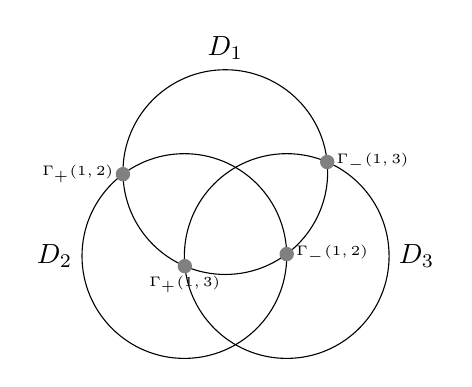
\begin{tikzpicture}[scale=1.3]
%\draw [help lines] (-5,-3) grid (5,3);

\draw[name path = c1] (0,0) circle (1cm);
\draw[name path = c3] (0.6,-0.82) circle (1cm);
\draw[name path = c2] (-0.4,-0.82) circle (1cm);

\node[above] at (0, 1) {$D_1$};
\node[left] at (-1.4, -0.82) {$D_2$};
\node[right] at (1.6, -0.82) {$D_3$};

\path [name intersections={of=c1 and c3}] ;
\foreach \i in {1,...,2}
\fill [color=gray] (intersection-\i) circle (2pt) ;

\node[right] at (intersection-1) {\tiny $\Gamma_-(1,3)$};
\node[left, below] at (intersection-2) {\tiny $\Gamma_+(1,3)$};

\path [name intersections={of=c1 and c2}] ;
\foreach \i in {1,...,2}
\fill [color=gray] (intersection-\i) circle (2pt) ;

\node[left] at (intersection-1) {\tiny $\Gamma_+(1,2)$};
\node[below,right] at (intersection-2) {\tiny $\Gamma_-(1,2)$};

%\draw [-] (-5,0) -- (5,0);
%\draw [-] (0,-3) -- (0,3);
%\draw [|-|] (0.001,-0.1) -- (4.999,-0.1);
\end{tikzpicture}
		%\fautor
		\label{fig:3disks_intersect}
	\end{figure}
\end{frame}

\begin{frame}{Maximum Weight Clique Problem}{Algorithm}
	For a disk $D_i$, a counter-clockwise traversal visits every $\Gamma_+(i,j)$ and $\Gamma_-(i,j)$ in counter-clockwise order.
	
	\begin{itemize}
		\item An intersection region of disks is bounded by arcs.
		
		\item The arc $\Gamma_+(i,j),\Gamma_-(i,j)$ (counter-clockwise) determines a region where $i$ and $j$ intersect.
		
		\item In a counter-clockwise traversal, the arcs where $\Gamma_+(i,j) > \Gamma_-(i,j)$ can be a problem for the implementation. Work-around: repeat it.
	\end{itemize}
\end{frame}

\begin{frame}{Maximum Weight Clique Problem}{Algorithm}
	
	The algorithm is described simply as:
	
	For every disk, traverse the sorted list of intersection angles twice, keeping a set of active disks, and the current best solution.
	
\begin{figure}[H]
	\centering
	
	\caption{The intersections list of a disk with three other disks.}
	\tikzset{every picture/.style={line width=0.75pt}} %set default line width to 0.75pt        

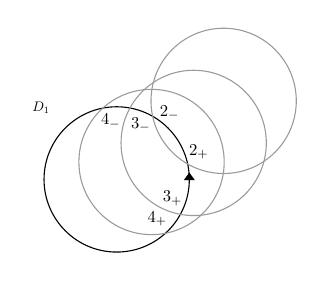
\begin{tikzpicture}[x=0.75pt,y=0.75pt,yscale=-1.4,xscale=1.4]
%uncomment if require: \path (0,95); %set diagram left start at 0, and has height of 95

%Shape: Circle [id:dp37777408295388804] 
\draw   (21,59.5) .. controls (21,45.69) and (32.19,34.5) .. (46,34.5) .. controls (59.81,34.5) and (71,45.69) .. (71,59.5) .. controls (71,73.31) and (59.81,84.5) .. (46,84.5) .. controls (32.19,84.5) and (21,73.31) .. (21,59.5) -- cycle ;
%Shape: Circle [id:dp4562198988843913] 
\draw  [color={rgb, 255:red, 155; green, 155; blue, 155 }  ,draw opacity=1 ] (47.5,46.94) .. controls (47.5,33.14) and (58.69,21.94) .. (72.5,21.94) .. controls (86.31,21.94) and (97.5,33.14) .. (97.5,46.94) .. controls (97.5,60.75) and (86.31,71.94) .. (72.5,71.94) .. controls (58.69,71.94) and (47.5,60.75) .. (47.5,46.94) -- cycle ;
%Shape: Circle [id:dp8913971633985722] 
\draw  [color={rgb, 255:red, 155; green, 155; blue, 155 }  ,draw opacity=1 ] (33,53.5) .. controls (33,39.69) and (44.19,28.5) .. (58,28.5) .. controls (71.81,28.5) and (83,39.69) .. (83,53.5) .. controls (83,67.31) and (71.81,78.5) .. (58,78.5) .. controls (44.19,78.5) and (33,67.31) .. (33,53.5) -- cycle ;
%Shape: Circle [id:dp05970043129919356] 
\draw  [color={rgb, 255:red, 155; green, 155; blue, 155 }  ,draw opacity=1 ] (57.81,32.47) .. controls (57.81,18.66) and (69,7.47) .. (82.81,7.47) .. controls (96.62,7.47) and (107.81,18.66) .. (107.81,32.47) .. controls (107.81,46.27) and (96.62,57.47) .. (82.81,57.47) .. controls (69,57.47) and (57.81,46.27) .. (57.81,32.47) -- cycle ;
%Straight Lines [id:da04725899028195979] 
%\draw[densely dotted]  (21,59.5) -- (71,59.5) ;


%Flowchart: Extract [id:dp5267407418119328] 
\draw  [fill={rgb, 255:red, 0; green, 0; blue, 0 }  ,fill opacity=1 ] (71,57.45) -- (72.52,59.55) -- (69.48,59.55) -- cycle ;

\draw (60,73) node [scale=0.6]  {$4_+$};
% Text Node
\draw (65.22,66) node [scale=0.6]  {$3_+$};
% Text Node
\draw (74.22,50) node [scale=0.6]  {$2_+$};
% Text Node
\draw (64.22,36.56) node [scale=0.6]  {$2_-$};
% Text Node
\draw (54.32,40.66) node [scale=0.6]  {$3_-$};
% Text Node
\draw (44.02,39.56) node [scale=0.6]  {$4_-$};


% Text Node
\draw (20,35) node [scale=0.5]  {$D_{1}$};
\end{tikzpicture}

\begin{tikzpicture}

\matrix [matrix of nodes,row sep=,row sep=0mm,
column 1/.style={nodes={rectangle,draw,minimum width=1.5em, minimum height=0.5em}},
column 2/.style={nodes={rectangle,draw,minimum width=1.5em, minimum height=0.5em}},
column 3/.style={nodes={rectangle,draw,minimum width=1.5em, minimum height=0.5em}},
column 4/.style={nodes={rectangle,draw,minimum width=1.5em, minimum height=0.5em}},
column 5/.style={nodes={rectangle,draw,minimum width=1.5em, minimum height=0.5em}},
column 6/.style={nodes={rectangle,draw,minimum width=1.5em, minimum height=0.5em}},
column 7/.style={nodes={rectangle,draw,minimum width=1.5em, color=gray, minimum height=0.5em}},
column 8/.style={nodes={rectangle,draw,minimum width=1.5em, color=gray, minimum height=0.5em}},
column 9/.style={nodes={rectangle,draw,minimum width=1.5em, color=gray, minimum height=0.5em}},
column 10/.style={nodes={rectangle,draw,minimum width=1.5em, color=gray, minimum height=0.5em}},
column 11/.style={nodes={rectangle,draw,minimum width=1.5em, color=gray, minimum height=0.5em}},
column 12/.style={nodes={rectangle,draw,minimum width=1.5em, color=gray, minimum height=0.5em}}
] (O)
{
$2_+$ & $2_-$ & $3_-$ & $4_-$ & $4_+$ & $3_+$ & $2_+$ & $2_-$ & $3_-$ & $4_-$ & $4_+$ & $3_+$\\
%$+$ & $-$ & $-$ & $-$ & $+$ & $+$\\
};

\node at (-4,-0.5) {$0$};
\node at (0,-0.5) {$2\pi$};
\end{tikzpicture}
%	\fautor
	\label{fig:array_disks}
\end{figure}
\end{frame}

\begin{frame}{Maximum Weight Clique Problem}{Algorithm}
\begin{figure}
	%\centering
	
	\caption{A traversal for $D_1$ with green disks representing the active set and red signs representing the current angle being visited (some are omitted).}
	\usetikzlibrary{matrix}



\tikzset{every picture/.style={line width=0.75pt}} %set default line width to 0.75pt        

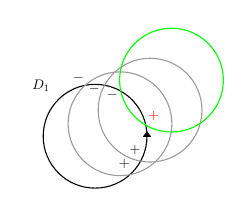
\begin{tikzpicture}[x=0.75pt,y=0.75pt,yscale=-1,xscale=1]
%uncomment if require: \path (0,95); %set diagram left start at 0, and has height of 95

%Shape: Circle [id:dp37777408295388804] 
\draw   (21,59.5) .. controls (21,45.69) and (32.19,34.5) .. (46,34.5) .. controls (59.81,34.5) and (71,45.69) .. (71,59.5) .. controls (71,73.31) and (59.81,84.5) .. (46,84.5) .. controls (32.19,84.5) and (21,73.31) .. (21,59.5) -- cycle ;
%Shape: Circle [id:dp4562198988843913] 
\draw  [color={rgb, 255:red, 155; green, 155; blue, 155 }  ,draw opacity=1 ] (47.5,46.94) .. controls (47.5,33.14) and (58.69,21.94) .. (72.5,21.94) .. controls (86.31,21.94) and (97.5,33.14) .. (97.5,46.94) .. controls (97.5,60.75) and (86.31,71.94) .. (72.5,71.94) .. controls (58.69,71.94) and (47.5,60.75) .. (47.5,46.94) -- cycle ;
%Shape: Circle [id:dp8913971633985722] 
\draw  [color={rgb, 255:red, 155; green, 155; blue, 155 }  ,draw opacity=1 ] (33,53.5) .. controls (33,39.69) and (44.19,28.5) .. (58,28.5) .. controls (71.81,28.5) and (83,39.69) .. (83,53.5) .. controls (83,67.31) and (71.81,78.5) .. (58,78.5) .. controls (44.19,78.5) and (33,67.31) .. (33,53.5) -- cycle ;
%Shape: Circle [id:dp05970043129919356] 
\draw  [color=green  ,draw opacity=1 ] (57.81,32.47) .. controls (57.81,18.66) and (69,7.47) .. (82.81,7.47) .. controls (96.62,7.47) and (107.81,18.66) .. (107.81,32.47) .. controls (107.81,46.27) and (96.62,57.47) .. (82.81,57.47) .. controls (69,57.47) and (57.81,46.27) .. (57.81,32.47) -- cycle ;
%Straight Lines [id:da04725899028195979] 
%\draw[densely dotted]  (21,59.5) -- (71,59.5) ;


%Flowchart: Extract [id:dp5267407418119328] 
\draw  [fill={rgb, 255:red, 0; green, 0; blue, 0 }  ,fill opacity=1 ] (71,57.45) -- (72.52,59.55) -- (69.48,59.55) -- cycle ;

\draw (60,73) node [scale=0.5]  {$+$};
% Text Node
\draw (65.22,66) node [scale=0.5]  {$+$};
% Text Node
\draw (74.22,50) node [scale=0.5,color=red]  {$+$};
% Text Node
\draw (54.22,39.56) node [scale=0.5]  {$-$};
% Text Node
\draw (45.62,36.96) node [scale=0.5]  {$-$};
% Text Node
\draw (38.02,31.56) node [scale=0.5]  {$-$};


% Text Node
\draw (20,35) node [scale=0.5]  {$D_{1}$};
\end{tikzpicture}
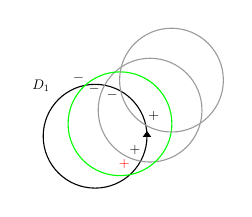
\begin{tikzpicture}[x=0.75pt,y=0.75pt,yscale=-1,xscale=1]
%uncomment if require: \path (0,95); %set diagram left start at 0, and has height of 95

%Shape: Circle [id:dp37777408295388804] 
\draw   (21,59.5) .. controls (21,45.69) and (32.19,34.5) .. (46,34.5) .. controls (59.81,34.5) and (71,45.69) .. (71,59.5) .. controls (71,73.31) and (59.81,84.5) .. (46,84.5) .. controls (32.19,84.5) and (21,73.31) .. (21,59.5) -- cycle ;
%Shape: Circle [id:dp4562198988843913] 
\draw  [color={rgb, 255:red, 155; green, 155; blue, 155 }  ,draw opacity=1 ] (47.5,46.94) .. controls (47.5,33.14) and (58.69,21.94) .. (72.5,21.94) .. controls (86.31,21.94) and (97.5,33.14) .. (97.5,46.94) .. controls (97.5,60.75) and (86.31,71.94) .. (72.5,71.94) .. controls (58.69,71.94) and (47.5,60.75) .. (47.5,46.94) -- cycle ;
%Shape: Circle [id:dp8913971633985722] 
\draw  [color=green  ,draw opacity=1 ] (33,53.5) .. controls (33,39.69) and (44.19,28.5) .. (58,28.5) .. controls (71.81,28.5) and (83,39.69) .. (83,53.5) .. controls (83,67.31) and (71.81,78.5) .. (58,78.5) .. controls (44.19,78.5) and (33,67.31) .. (33,53.5) -- cycle ;
%Shape: Circle [id:dp05970043129919356] 
\draw  [color={rgb, 255:red, 155; green, 155; blue, 155 }  ,draw opacity=1 ] (57.81,32.47) .. controls (57.81,18.66) and (69,7.47) .. (82.81,7.47) .. controls (96.62,7.47) and (107.81,18.66) .. (107.81,32.47) .. controls (107.81,46.27) and (96.62,57.47) .. (82.81,57.47) .. controls (69,57.47) and (57.81,46.27) .. (57.81,32.47) -- cycle ;
%Straight Lines [id:da04725899028195979] 
%\draw[densely dotted]  (21,59.5) -- (71,59.5) ;


%Flowchart: Extract [id:dp5267407418119328] 
\draw  [fill={rgb, 255:red, 0; green, 0; blue, 0 }  ,fill opacity=1 ] (71,57.45) -- (72.52,59.55) -- (69.48,59.55) -- cycle ;

\draw (60,73) node [scale=0.5,color=red]  {$+$};
% Text Node
\draw (65.22,66) node [scale=0.5]  {$+$};
% Text Node
\draw (74.22,50) node [scale=0.5]  {$+$};
% Text Node
\draw (54.22,39.56) node [scale=0.5]  {$-$};
% Text Node
\draw (45.62,36.96) node [scale=0.5]  {$-$};
% Text Node
\draw (38.02,31.56) node [scale=0.5]  {$-$};


% Text Node
\draw (20,35) node [scale=0.5]  {$D_{1}$};
\end{tikzpicture}
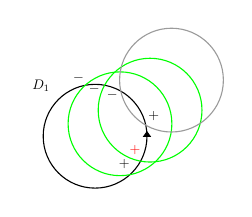
\begin{tikzpicture}[x=0.75pt,y=0.75pt,yscale=-1,xscale=1]
%uncomment if require: \path (0,95); %set diagram left start at 0, and has height of 95

%Shape: Circle [id:dp37777408295388804] 
\draw   (21,59.5) .. controls (21,45.69) and (32.19,34.5) .. (46,34.5) .. controls (59.81,34.5) and (71,45.69) .. (71,59.5) .. controls (71,73.31) and (59.81,84.5) .. (46,84.5) .. controls (32.19,84.5) and (21,73.31) .. (21,59.5) -- cycle ;


%Shape: Circle [id:dp4562198988843913] 
\draw  [color=green  ,draw opacity=1 ] (47.5,46.94) .. controls (47.5,33.14) and (58.69,21.94) .. (72.5,21.94) .. controls (86.31,21.94) and (97.5,33.14) .. (97.5,46.94) .. controls (97.5,60.75) and (86.31,71.94) .. (72.5,71.94) .. controls (58.69,71.94) and (47.5,60.75) .. (47.5,46.94) -- cycle ;


%Shape: Circle [id:dp8913971633985722] 
\draw  [color=green  ,draw opacity=1 ] (33,53.5) .. controls (33,39.69) and (44.19,28.5) .. (58,28.5) .. controls (71.81,28.5) and (83,39.69) .. (83,53.5) .. controls (83,67.31) and (71.81,78.5) .. (58,78.5) .. controls (44.19,78.5) and (33,67.31) .. (33,53.5) -- cycle ;


%Shape: Circle [id:dp05970043129919356] 
\draw  [color={rgb, 255:red, 155; green, 155; blue, 155 }  ,draw opacity=1 ] (57.81,32.47) .. controls (57.81,18.66) and (69,7.47) .. (82.81,7.47) .. controls (96.62,7.47) and (107.81,18.66) .. (107.81,32.47) .. controls (107.81,46.27) and (96.62,57.47) .. (82.81,57.47) .. controls (69,57.47) and (57.81,46.27) .. (57.81,32.47) -- cycle ;
%Straight Lines [id:da04725899028195979] 
%\draw[densely dotted]  (21,59.5) -- (71,59.5) ;


%Flowchart: Extract [id:dp5267407418119328] 
\draw  [fill={rgb, 255:red, 0; green, 0; blue, 0 }  ,fill opacity=1 ] (71,57.45) -- (72.52,59.55) -- (69.48,59.55) -- cycle ;

\draw (60,73) node [scale=0.5]  {$+$};
% Text Node
\draw (65.22,66) node [scale=0.5,color=red]  {$+$};
% Text Node
\draw (74.22,50) node [scale=0.5]  {$+$};
% Text Node
\draw (54.22,39.56) node [scale=0.5]  {$-$};
% Text Node
\draw (45.62,36.96) node [scale=0.5]  {$-$};
% Text Node
\draw (38.02,31.56) node [scale=0.5]  {$-$};


% Text Node
\draw (20,35) node [scale=0.5]  {$D_{1}$};
\end{tikzpicture}
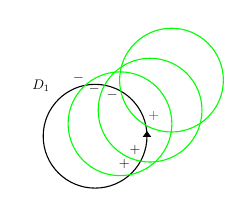
\begin{tikzpicture}[x=0.75pt,y=0.75pt,yscale=-1,xscale=1]
%uncomment if require: \path (0,95); %set diagram left start at 0, and has height of 95

%Shape: Circle [id:dp37777408295388804] 
\draw   (21,59.5) .. controls (21,45.69) and (32.19,34.5) .. (46,34.5) .. controls (59.81,34.5) and (71,45.69) .. (71,59.5) .. controls (71,73.31) and (59.81,84.5) .. (46,84.5) .. controls (32.19,84.5) and (21,73.31) .. (21,59.5) -- cycle ;


%Shape: Circle [id:dp4562198988843913] 
\draw  [color=green  ,draw opacity=1 ] (47.5,46.94) .. controls (47.5,33.14) and (58.69,21.94) .. (72.5,21.94) .. controls (86.31,21.94) and (97.5,33.14) .. (97.5,46.94) .. controls (97.5,60.75) and (86.31,71.94) .. (72.5,71.94) .. controls (58.69,71.94) and (47.5,60.75) .. (47.5,46.94) -- cycle ;


%Shape: Circle [id:dp8913971633985722] 
\draw  [color=green  ,draw opacity=1 ] (33,53.5) .. controls (33,39.69) and (44.19,28.5) .. (58,28.5) .. controls (71.81,28.5) and (83,39.69) .. (83,53.5) .. controls (83,67.31) and (71.81,78.5) .. (58,78.5) .. controls (44.19,78.5) and (33,67.31) .. (33,53.5) -- cycle ;


%Shape: Circle [id:dp05970043129919356] 
\draw  [color=green ,draw opacity=1 ] (57.81,32.47) .. controls (57.81,18.66) and (69,7.47) .. (82.81,7.47) .. controls (96.62,7.47) and (107.81,18.66) .. (107.81,32.47) .. controls (107.81,46.27) and (96.62,57.47) .. (82.81,57.47) .. controls (69,57.47) and (57.81,46.27) .. (57.81,32.47) -- cycle ;
%Straight Lines [id:da04725899028195979] 
%\draw[densely dotted]  (21,59.5) -- (71,59.5) ;


%Flowchart: Extract [id:dp5267407418119328] 
\draw  [fill={rgb, 255:red, 0; green, 0; blue, 0 }  ,fill opacity=1 ] (71,57.45) -- (72.52,59.55) -- (69.48,59.55) -- cycle ;

\draw (60,73) node [scale=0.5]  {$+$};
% Text Node
\draw (65.22,66) node [scale=0.5]  {$+$};
% Text Node
\draw (74.22,50) node [scale=0.5,color=red]  {$+$};
% Text Node
\draw (54.22,39.56) node [scale=0.5]  {$-$};
% Text Node
\draw (45.62,36.96) node [scale=0.5]  {$-$};
% Text Node
\draw (38.02,31.56) node [scale=0.5]  {$-$};


% Text Node
\draw (20,35) node [scale=0.5]  {$D_{1}$};
\end{tikzpicture}
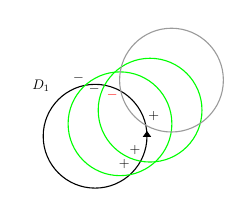
\begin{tikzpicture}[x=0.75pt,y=0.75pt,yscale=-1,xscale=1]
%uncomment if require: \path (0,95); %set diagram left start at 0, and has height of 95

%Shape: Circle [id:dp37777408295388804] 
\draw   (21,59.5) .. controls (21,45.69) and (32.19,34.5) .. (46,34.5) .. controls (59.81,34.5) and (71,45.69) .. (71,59.5) .. controls (71,73.31) and (59.81,84.5) .. (46,84.5) .. controls (32.19,84.5) and (21,73.31) .. (21,59.5) -- cycle ;


%Shape: Circle [id:dp4562198988843913] 
\draw  [color=green  ,draw opacity=1 ] (47.5,46.94) .. controls (47.5,33.14) and (58.69,21.94) .. (72.5,21.94) .. controls (86.31,21.94) and (97.5,33.14) .. (97.5,46.94) .. controls (97.5,60.75) and (86.31,71.94) .. (72.5,71.94) .. controls (58.69,71.94) and (47.5,60.75) .. (47.5,46.94) -- cycle ;


%Shape: Circle [id:dp8913971633985722] 
\draw  [color=green  ,draw opacity=1 ] (33,53.5) .. controls (33,39.69) and (44.19,28.5) .. (58,28.5) .. controls (71.81,28.5) and (83,39.69) .. (83,53.5) .. controls (83,67.31) and (71.81,78.5) .. (58,78.5) .. controls (44.19,78.5) and (33,67.31) .. (33,53.5) -- cycle ;


%Shape: Circle [id:dp05970043129919356] 
\draw  [color={rgb, 255:red, 155; green, 155; blue, 155 }  ,draw opacity=1 ] (57.81,32.47) .. controls (57.81,18.66) and (69,7.47) .. (82.81,7.47) .. controls (96.62,7.47) and (107.81,18.66) .. (107.81,32.47) .. controls (107.81,46.27) and (96.62,57.47) .. (82.81,57.47) .. controls (69,57.47) and (57.81,46.27) .. (57.81,32.47) -- cycle ;
%Straight Lines [id:da04725899028195979] 
%\draw[densely dotted]  (21,59.5) -- (71,59.5) ;


%Flowchart: Extract [id:dp5267407418119328] 
\draw  [fill={rgb, 255:red, 0; green, 0; blue, 0 }  ,fill opacity=1 ] (71,57.45) -- (72.52,59.55) -- (69.48,59.55) -- cycle ;

\draw (60,73) node [scale=0.5]  {$+$};
% Text Node
\draw (65.22,66) node [scale=0.5]  {$+$};
% Text Node
\draw (74.22,50) node [scale=0.5]  {$+$};
% Text Node
\draw (54.22,39.56) node [scale=0.5,color=red]  {$-$};
% Text Node
\draw (45.62,36.96) node [scale=0.5]  {$-$};
% Text Node
\draw (38.02,31.56) node [scale=0.5]  {$-$};


% Text Node
\draw (20,35) node [scale=0.5]  {$D_{1}$};
\end{tikzpicture}
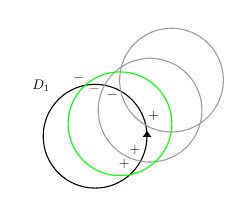
\begin{tikzpicture}[x=0.75pt,y=0.75pt,yscale=-1,xscale=1]
%uncomment if require: \path (0,95); %set diagram left start at 0, and has height of 95

%Shape: Circle [id:dp37777408295388804] 
\draw   (21,59.5) .. controls (21,45.69) and (32.19,34.5) .. (46,34.5) .. controls (59.81,34.5) and (71,45.69) .. (71,59.5) .. controls (71,73.31) and (59.81,84.5) .. (46,84.5) .. controls (32.19,84.5) and (21,73.31) .. (21,59.5) -- cycle ;


%Shape: Circle [id:dp4562198988843913] 
\draw  [color={rgb, 255:red, 155; green, 155; blue, 155 },draw opacity=1 ] (47.5,46.94) .. controls (47.5,33.14) and (58.69,21.94) .. (72.5,21.94) .. controls (86.31,21.94) and (97.5,33.14) .. (97.5,46.94) .. controls (97.5,60.75) and (86.31,71.94) .. (72.5,71.94) .. controls (58.69,71.94) and (47.5,60.75) .. (47.5,46.94) -- cycle ;


%Shape: Circle [id:dp8913971633985722] 
\draw  [color=green  ,draw opacity=1 ] (33,53.5) .. controls (33,39.69) and (44.19,28.5) .. (58,28.5) .. controls (71.81,28.5) and (83,39.69) .. (83,53.5) .. controls (83,67.31) and (71.81,78.5) .. (58,78.5) .. controls (44.19,78.5) and (33,67.31) .. (33,53.5) -- cycle ;


%Shape: Circle [id:dp05970043129919356] 
\draw  [color={rgb, 255:red, 155; green, 155; blue, 155 }  ,draw opacity=1 ] (57.81,32.47) .. controls (57.81,18.66) and (69,7.47) .. (82.81,7.47) .. controls (96.62,7.47) and (107.81,18.66) .. (107.81,32.47) .. controls (107.81,46.27) and (96.62,57.47) .. (82.81,57.47) .. controls (69,57.47) and (57.81,46.27) .. (57.81,32.47) -- cycle ;
%Straight Lines [id:da04725899028195979] 
%\draw[densely dotted]  (21,59.5) -- (71,59.5) ;


%Flowchart: Extract [id:dp5267407418119328] 
\draw  [fill={rgb, 255:red, 0; green, 0; blue, 0 }  ,fill opacity=1 ] (71,57.45) -- (72.52,59.55) -- (69.48,59.55) -- cycle ;

\draw (60,73) node [scale=0.5]  {$+$};
% Text Node
\draw (65.22,66) node [scale=0.5]  {$+$};
% Text Node
\draw (74.22,50) node [scale=0.5]  {$+$};
% Text Node
\draw (54.22,39.56) node [scale=0.5]  {$-$};
% Text Node
\draw (45.62,36.96) node [scale=0.5,color=red]  {$-$};
% Text Node
\draw (38.02,31.56) node [scale=0.5]  {$-$};


% Text Node
\draw (20,35) node [scale=0.5]  {$D_{1}$};
\end{tikzpicture}
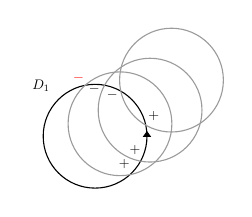
\begin{tikzpicture}[x=0.75pt,y=0.75pt,yscale=-1,xscale=1]
%uncomment if require: \path (0,95); %set diagram left start at 0, and has height of 95

%Shape: Circle [id:dp37777408295388804] 
\draw   (21,59.5) .. controls (21,45.69) and (32.19,34.5) .. (46,34.5) .. controls (59.81,34.5) and (71,45.69) .. (71,59.5) .. controls (71,73.31) and (59.81,84.5) .. (46,84.5) .. controls (32.19,84.5) and (21,73.31) .. (21,59.5) -- cycle ;


%Shape: Circle [id:dp4562198988843913] 
\draw  [color={rgb, 255:red, 155; green, 155; blue, 155 },draw opacity=1 ] (47.5,46.94) .. controls (47.5,33.14) and (58.69,21.94) .. (72.5,21.94) .. controls (86.31,21.94) and (97.5,33.14) .. (97.5,46.94) .. controls (97.5,60.75) and (86.31,71.94) .. (72.5,71.94) .. controls (58.69,71.94) and (47.5,60.75) .. (47.5,46.94) -- cycle ;


%Shape: Circle [id:dp8913971633985722] 
\draw  [color={rgb, 255:red, 155; green, 155; blue, 155 } ,draw opacity=1 ] (33,53.5) .. controls (33,39.69) and (44.19,28.5) .. (58,28.5) .. controls (71.81,28.5) and (83,39.69) .. (83,53.5) .. controls (83,67.31) and (71.81,78.5) .. (58,78.5) .. controls (44.19,78.5) and (33,67.31) .. (33,53.5) -- cycle ;


%Shape: Circle [id:dp05970043129919356] 
\draw  [color={rgb, 255:red, 155; green, 155; blue, 155 }  ,draw opacity=1 ] (57.81,32.47) .. controls (57.81,18.66) and (69,7.47) .. (82.81,7.47) .. controls (96.62,7.47) and (107.81,18.66) .. (107.81,32.47) .. controls (107.81,46.27) and (96.62,57.47) .. (82.81,57.47) .. controls (69,57.47) and (57.81,46.27) .. (57.81,32.47) -- cycle ;
%Straight Lines [id:da04725899028195979] 
%\draw[densely dotted]  (21,59.5) -- (71,59.5) ;


%Flowchart: Extract [id:dp5267407418119328] 
\draw  [fill={rgb, 255:red, 0; green, 0; blue, 0 }  ,fill opacity=1 ] (71,57.45) -- (72.52,59.55) -- (69.48,59.55) -- cycle ;

\draw (60,73) node [scale=0.5]  {$+$};
% Text Node
\draw (65.22,66) node [scale=0.5]  {$+$};
% Text Node
\draw (74.22,50) node [scale=0.5]  {$+$};
% Text Node
\draw (54.22,39.56) node [scale=0.5]  {$-$};
% Text Node
\draw (45.62,36.96) node [scale=0.5]  {$-$};
% Text Node
\draw (38.02,31.56) node [scale=0.5,color=red]  {\textbf{$-$}};


% Text Node
\draw (20,35) node [scale=0.5]  {$D_{1}$};
\end{tikzpicture}



	%	\fautor
	%\label{fig:array_disks}
\end{figure}
\end{frame}


\begin{frame}{Maximum Weight Clique Problem}{Algorithm}
	
	The run-time complexity of the algorithm is $\bigO(n^2\log{n})$.
	
	\begin{itemize}
		\item There are $\bigO(n^2)$ intersections among $n$ disks
		
		\item Sorting takes $\bigO(n^2\log{n})$
		
		\item The traversal takes $\bigO(n)$ for every disk.
		
		\item It can be implemented in $K\log{n}$ where $K$ is the number of intersections.
	\end{itemize}

\begin{block}{Multiple disks}
	For every disk, try every possible assignment that the traversal goes through. \cite{cabello:2006} proposed a $\bigO(n^{2m-1})$ algorithm.
\end{block}
	

	
	
\end{frame}

\section{Maximal Covering by Ellipses}

\begin{frame}{Maximal Covering by Ellipses}
	Let $MCE(\Pp, a, b)$ be an instance of the maximal covering by one ellipse, with $E$ being an ellipse with shape parameters $(a,b) \in \R_{>0}^2$, an optimal solution of $MCE(\Pp, a, b)$ is given by
	
	\begin{equation*}
	\max_q |\Pp \cap (q)|,
	\end{equation*}

	\begin{itemize}
		\item $E(q)$ is an axis-parallel ellipse with center point $q$
		\item Assuming unit weights for now
		\item Same algorithm for one disk
	\end{itemize}

\end{frame}

\begin{frame}{Maximal Covering by Ellipses}
\begin{figure}[H]
	\centering
	
	\caption{Intersection points of $E_1$ with $E_2$ and $E_3$ along with opening and closing angles indicators.}
	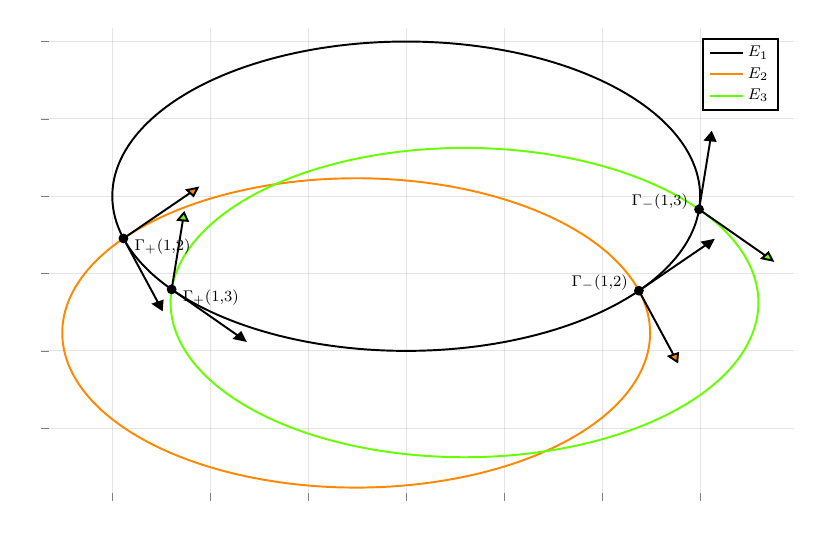
\begin{tikzpicture}[scale=0.7]
\begin{axis}[height = {101.6mm}, ylabel = {}, xmin = {-3.7279015473763786}, xmax = {3.956162987575968}, ymax = {2.172965670438345}, xlabel = {}, unbounded coords=jump,scaled x ticks = false,xlabel style = {font = {\fontsize{11 pt}{14.3 pt}\selectfont}, color = {rgb,1:red,0.00000000;green,0.00000000;blue,0.00000000}, draw opacity = 1.0, rotate = 0.0},xmajorgrids = true,xtick = {-3.0,-2.0,-1.0,0.0,1.0,2.0,3.0},xticklabels = {},xtick align = inside,xticklabel style = {font = {\fontsize{8 pt}{10.4 pt}\selectfont}, color = {rgb,1:red,0.00000000;green,0.00000000;blue,0.00000000}, draw opacity = 1.0, rotate = 0.0},x grid style = {color = {rgb,1:red,0.00000000;green,0.00000000;blue,0.00000000},
draw opacity = 0.1,
line width = 0.5,
solid},axis lines* = left,separate axis lines,x axis line style = {draw opacity = 0},scaled y ticks = false,ylabel style = {font = {\fontsize{11 pt}{14.3 pt}\selectfont}, color = {rgb,1:red,0.00000000;green,0.00000000;blue,0.00000000}, draw opacity = 1.0, rotate = 0.0},ymajorgrids = true,ytick = {-3.0,-2.0,-1.0,0.0,1.0,2.0},yticklabels = {},ytick align = inside,yticklabel style = {font = {\fontsize{8 pt}{10.4 pt}\selectfont}, color = {rgb,1:red,0.00000000;green,0.00000000;blue,0.00000000}, draw opacity = 1.0, rotate = 0.0},y grid style = {color = {rgb,1:red,0.00000000;green,0.00000000;blue,0.00000000},
draw opacity = 0.1,
line width = 0.5,
solid},axis lines* = left,separate axis lines,y axis line style = {draw opacity = 0},    xshift = 0.0mm,
    yshift = 0.0mm,
    axis background/.style={fill={rgb,1:red,1.00000000;green,1.00000000;blue,1.00000000}}
,legend style = {color = {rgb,1:red,0.00000000;green,0.00000000;blue,0.00000000},
draw opacity = 1.0,
line width = 1,
solid,fill = {rgb,1:red,1.00000000;green,1.00000000;blue,1.00000000},font = {\fontsize{8 pt}{10.4 pt}\selectfont}},colorbar style={title=}, ymin = {-3.9406895045294608}, width = {152.4mm}]\addplot+ [color = {rgb,1:red,0.00000000;green,0.00000000;blue,0.00000000},
draw opacity = 1.0,
line width = 1,
solid,mark = none,
mark size = 2.0,
mark options = {
    color = {rgb,1:red,0.00000000;green,0.00000000;blue,0.00000000}, draw opacity = 1.0,
    fill = {rgb,1:red,0.00000000;green,0.00000000;blue,0.00000000}, fill opacity = 1.0,
    line width = 1,
    rotate = 0,
    solid
}]coordinates {
(3.0, 0.0)
(2.9985047673785212, 0.06313709952962106)
(2.99402055999448, 0.1262112626253473)
(2.9865518478033177, 0.18915961558968988)
(2.9761060757797733, 0.2519194101354351)
(2.962693656496571, 0.31442808593450156)
(2.9463279597449414, 0.37662333297943573)
(2.9270252992073207, 0.43844315369538267)
(2.9048049161955216, 0.4998259247406167)
(2.879688960470571, 0.5607104584340288)
(2.8517024681633485, 0.6210360637483376)
(2.8208733368180265, 0.6807426068082256)
(2.787232297583192, 0.7397705708330936)
(2.7508128845783664, 0.7980611154646818)
(2.7116514014664705, 0.8555561354204192)
(2.669786885265541, 0.9121983184140319)
(2.625261067435781, 0.9679312022856775)
(2.578118332280736, 1.0226992312846535)
(2.528405672704052, 1.076447811448577)
(2.4761726433659286, 1.1291233650238361)
(2.421471311285956, 1.1806733838730568)
(2.3643562039415773, 1.2310464818163585)
(2.3048842549139126, 1.2801924458542142)
(2.2431147471351274, 1.3280622862208624)
(2.1791092537939183, 1.3746082852183685)
(2.1129315769580166, 1.4197840447826657)
(2.0446476839749015, 1.4635445327341534)
(1.974325641714113, 1.505846127666754)
(1.902035548716716, 1.546646662430678)
(1.82784946531955, 1.5859054661655572)
(1.7518413418239187, 1.6235834048420414)
(1.6740869447803206, 1.6596429202714515)
(1.5946637814627043, 1.6940480675445977)
(1.5136510226075326, 1.7267645508624465)
(1.4311294234946685, 1.7577597577229207)
(1.3471812434487604, 1.7870027914297482)
(1.261890163841353, 1.8144645018909626)
(1.1753412046754794, 1.840117514676349)
(1.0876206398358734, 1.8639362583048695)
(0.9988159110892831, 1.885896989734874)
(0.9090155409206182, 1.9059778180316784)
(0.8183090442918096, 1.9241587261889257)
(0.7267868394113495, 1.9404215910819727)
(0.6345401576034572, 1.9547502015334144)
(0.541660952366707, 1.9671302744727397)
(0.4482418077127828, 1.9775494691740052)
(0.35437584587672416, 1.9859973995573392)
(0.26015663449065285, 1.9924656445420135)
(0.1656780933135245, 1.9969477564407576)
(0.0710344006098723, 1.9994392673869559)
(-0.02368010072913993, 1.9999376937883127)
(-0.1183709972287581, 1.9984425388025513)
(-0.21294389894404733, 1.9949552928326777)
(-0.3073045335498399, 1.9894794320413138)
(-0.40135884031343716, 1.9820204148855842)
(-0.49501306385639726, 1.9725856766760055)
(-0.588173847611934, 1.9611846221648082)
(-0.68074832688477, 1.9478286161710756)
(-0.7726442214206901, 1.9325309722520436)
(-0.8637699273934991, 1.9153069394318591)
(-0.9540346087177143, 1.896173687001019)
(-1.043348287595947, 1.8751502874016501)
(-1.1316219342107279, 1.8522576972156826)
(-1.2187675554713666, 1.8275187362748735)
(-1.304698282727379, 1.8009580649135033)
(-1.389328458361043, 1.7726021593864174)
(-1.4725737211727805, 1.7424792854769193)
(-1.5543510904742317, 1.710619470320824)
(-1.6345790488052114, 1.6770544724747547)
(-1.713177623192084, 1.6418177502585252)
(-1.7900684648665677, 1.604944428403156)
(-1.8651749273654852, 1.566471263037781)
(-1.9384221429336286, 1.5264366050503373)
(-2.009737097153566, 1.484880361858566)
(-2.079048701727995, 1.4418439576294326)
(-2.1462878653421136, 1.3973702919866131)
(-2.2113875625353363, 1.3515036972472176)
(-2.274282900513736, 1.3042898942303736)
(-2.3349111838365904, 1.2557759466817167)
(-2.393211976912558, 1.206010214359229)
(-2.449127164243197, 1.1550423048271772)
(-2.502601008353752, 1.1029230240062151)
(-2.5535802053534837, 1.0497043255289369)
(-2.6020139380701437, 0.9954392589513668)
(-2.6478539267056407, 0.9401819168720059)
(-2.6910544769623908, 0.8839873810111583)
(-2.7315725255923864, 0.8269116673042683)
(-2.7693676833235816, 0.769011670064022)
(-2.8044022751207947, 0.7103451052668572)
(-2.8366413777410013, 0.6509704530204232)
(-2.8660528545455843, 0.5909468992693401)
(-2.8926073875348353, 0.5303342767973575)
(-2.916278506572771, 0.46919300558473775)
(-2.9370426157731435, 0.4075840325803047)
(-2.954879017020331, 0.3455687709481997)
(-2.9697699306016716, 0.28320903884990317)
(-2.9817005129306633, 0.22056699782255015)
(-2.9906588713433795, 0.1577050908149532)
(-2.996636075953331, 0.09468597994311641)
(-2.9996261685529717, 0.03157248402727453)
(-2.9996261685529717, -0.031572484027274035)
(-2.996636075953331, -0.09468597994311592)
(-2.9906588713433795, -0.1577050908149527)
(-2.9817005129306637, -0.22056699782254965)
(-2.9697699306016716, -0.2832090388499027)
(-2.9548790170203314, -0.34556877094819927)
(-2.9370426157731435, -0.40758403258030423)
(-2.916278506572771, -0.46919300558473725)
(-2.8926073875348353, -0.530334276797357)
(-2.866052854545585, -0.5909468992693396)
(-2.8366413777410013, -0.6509704530204228)
(-2.804402275120795, -0.7103451052668568)
(-2.769367683323582, -0.7690116700640215)
(-2.7315725255923864, -0.8269116673042679)
(-2.6910544769623908, -0.8839873810111578)
(-2.647853926705641, -0.9401819168720055)
(-2.6020139380701437, -0.9954392589513663)
(-2.5535802053534837, -1.0497043255289367)
(-2.5026010083537527, -1.1029230240062147)
(-2.4491271642431975, -1.155042304827177)
(-2.393211976912559, -1.2060102143592286)
(-2.3349111838365904, -1.2557759466817162)
(-2.274282900513737, -1.3042898942303731)
(-2.211387562535337, -1.3515036972472174)
(-2.1462878653421145, -1.3973702919866127)
(-2.079048701727996, -1.4418439576294324)
(-2.0097370971535664, -1.4848803618585658)
(-1.9384221429336304, -1.5264366050503364)
(-1.8651749273654858, -1.5664712630377808)
(-1.7900684648665695, -1.604944428403155)
(-1.713177623192085, -1.641817750258525)
(-1.634579048805211, -1.677054472474755)
(-1.5543510904742333, -1.7106194703208233)
(-1.4725737211727812, -1.742479285476919)
(-1.389328458361045, -1.7726021593864167)
(-1.3046982827273796, -1.800958064913503)
(-1.2187675554713666, -1.8275187362748735)
(-1.131621934210729, -1.8522576972156821)
(-1.0433482875959472, -1.8751502874016501)
(-0.9540346087177163, -1.8961736870010186)
(-0.8637699273935, -1.915306939431859)
(-0.7726442214206894, -1.9325309722520438)
(-0.6807483268847714, -1.9478286161710754)
(-0.5881738476119341, -1.9611846221648082)
(-0.4950130638563993, -1.9725856766760053)
(-0.4013588403134378, -1.9820204148855842)
(-0.3073045335498393, -1.989479432041314)
(-0.2129438989440487, -1.9949552928326775)
(-0.11837099722875816, -1.9984425388025513)
(-0.023680100729141333, -1.9999376937883127)
(0.07103440060987157, -1.9994392673869559)
(0.1656780933135251, -1.9969477564407576)
(0.2601566344906514, -1.9924656445420135)
(0.3543758458767241, -1.9859973995573392)
(0.44824180771278144, -1.9775494691740052)
(0.5416609523667063, -1.96713027447274)
(0.6345401576034577, -1.9547502015334144)
(0.7267868394113488, -1.9404215910819727)
(0.8183090442918095, -1.9241587261889257)
(0.9090155409206169, -1.9059778180316789)
(0.998815911089283, -1.885896989734874)
(1.0876206398358716, -1.8639362583048702)
(1.1753412046754788, -1.840117514676349)
(1.261890163841353, -1.8144645018909626)
(1.3471812434487593, -1.7870027914297486)
(1.4311294234946685, -1.7577597577229207)
(1.5136510226075308, -1.7267645508624474)
(1.5946637814627036, -1.694048067544598)
(1.6740869447803208, -1.6596429202714515)
(1.7518413418239178, -1.6235834048420419)
(1.82784946531955, -1.5859054661655572)
(1.9020355487167147, -1.546646662430679)
(1.9743256417141124, -1.5058461276667543)
(2.044647683974902, -1.4635445327341534)
(2.1129315769580157, -1.4197840447826664)
(2.179109253793918, -1.3746082852183685)
(2.243114747135126, -1.3280622862208633)
(2.3048842549139117, -1.2801924458542147)
(2.3643562039415773, -1.231046481816358)
(2.4214713112859556, -1.1806733838730574)
(2.4761726433659286, -1.1291233650238361)
(2.528405672704051, -1.076447811448578)
(2.5781183322807357, -1.0226992312846537)
(2.6252610674357815, -0.9679312022856771)
(2.66978688526554, -0.9121983184140325)
(2.7116514014664705, -0.8555561354204191)
(2.750812884578366, -0.7980611154646828)
(2.7872322975831914, -0.7397705708330939)
(2.820873336818026, -0.680742606808227)
(2.8517024681633485, -0.6210360637483382)
(2.879688960470571, -0.5607104584340287)
(2.904804916195521, -0.4998259247406176)
(2.9270252992073207, -0.4384431536953829)
(2.946327959744941, -0.37662333297943695)
(2.9626936564965707, -0.3144280859345021)
(2.9761060757797737, -0.25191941013543495)
(2.9865518478033177, -0.18915961558969077)
(2.99402055999448, -0.12621126262534743)
(2.9985047673785212, -0.06313709952962226)
(3.0, -4.898587196589413e-16)
};
\addlegendentry{$E_1$}
\addplot+ [color = {rgb,1:red,1.00000000;green,0.53160000;blue,0.00000000},
draw opacity = 1.0,
line width = 1,
solid,mark = none,
mark size = 2.0,
mark options = {
    color = {rgb,1:red,0.00000000;green,0.00000000;blue,0.00000000}, draw opacity = 1.0,
    fill = {rgb,1:red,1.00000000;green,0.53160000;blue,0.00000000}, fill opacity = 1.0,
    line width = 1,
    rotate = 0,
    solid
}]coordinates {
(2.489198145750716, -1.7677238340911159)
(2.487702913129237, -1.704586734561495)
(2.483218705745196, -1.6415125714657686)
(2.4757499935540337, -1.578564218501426)
(2.4653042215304892, -1.5158044239556807)
(2.451891802247287, -1.4532957481566142)
(2.4355261054956574, -1.3911005011116802)
(2.4162234449580366, -1.3292806803957333)
(2.3940030619462376, -1.2678979093504992)
(2.368887106221287, -1.207013375657087)
(2.3409006139140645, -1.1466877703427782)
(2.3100714825687425, -1.0869812272828903)
(2.2764304433339078, -1.0279532632580222)
(2.2400110303290823, -0.969662718626434)
(2.2008495472171865, -0.9121676986706967)
(2.158985031016257, -0.855525515677084)
(2.114459213186497, -0.7997926318054384)
(2.067316478031452, -0.7450246028064624)
(2.0176038184547678, -0.691276022642539)
(1.9653707891166445, -0.6386004690672797)
(1.910669457036672, -0.5870504502180591)
(1.8535543496922933, -0.5366773522747574)
(1.7940824006646285, -0.4875313882369017)
(1.7323128928858433, -0.43966154787025347)
(1.6683073995446343, -0.39311554887274736)
(1.6021297227087326, -0.34793978930845015)
(1.5338458297256174, -0.3041793013569625)
(1.4635237874648293, -0.2618777064243618)
(1.3912336944674322, -0.22107717166043783)
(1.317047611070266, -0.18181836792555872)
(1.2410394875746347, -0.14414042924907444)
(1.1632850905310366, -0.10808091381966434)
(1.0838619272134205, -0.0736757665465182)
(1.0028491683582486, -0.040959283228669374)
(0.9203275692453846, -0.009964076368195185)
(0.8363793891994765, 0.019278957338632274)
(0.7510883095920692, 0.04674066779984676)
(0.6645393504261955, 0.07239368058523321)
(0.5768187855865895, 0.09621242421375364)
(0.4880140568399992, 0.11817315564375819)
(0.3982136866713343, 0.13825398394056254)
(0.3075071900425257, 0.1564348920978098)
(0.21598498516206555, 0.17269775699085677)
(0.12373830335417324, 0.1870263674422985)
(0.030859098117423045, 0.1994064403816238)
(-0.0625600465365011, 0.20982563508288932)
(-0.15642600837255977, 0.21827356546622334)
(-0.2506452197586311, 0.22474181045089758)
(-0.3451237609357594, 0.22922392234964173)
(-0.4397674536394116, 0.23171543329584)
(-0.5344819549784239, 0.23221385969719677)
(-0.629172851478042, 0.2307187047114354)
(-0.7237457531933312, 0.2272314587415618)
(-0.8181063877991238, 0.22175559795019795)
(-0.9121606945627211, 0.21429658079446834)
(-1.0058149181056812, 0.2048618425848896)
(-1.0989757018612178, 0.19346078807369227)
(-1.1915501811340539, 0.18010478207995972)
(-1.283446075669974, 0.16480713816092774)
(-1.374571781642783, 0.14758310534074326)
(-1.464836462966998, 0.12844985290990318)
(-1.554150141845231, 0.10742645331053424)
(-1.642423788460012, 0.08453386312456668)
(-1.7295694097206504, 0.0597949021837576)
(-1.815500136976663, 0.03323423082238741)
(-1.9001303126103268, 0.004878325295301522)
(-1.9833755754220643, -0.02524454861419656)
(-2.0651529447235157, -0.05710436377029193)
(-2.1453809030544955, -0.09066936161636119)
(-2.223979477441368, -0.12590608383259072)
(-2.3008703191158517, -0.1627794056879599)
(-2.375976781614769, -0.20125257105333483)
(-2.4492239971829126, -0.2412872290407786)
(-2.52053895140285, -0.2828434722325499)
(-2.589850555977279, -0.32587987646168326)
(-2.6570897195913976, -0.3703535421045028)
(-2.7221894167846203, -0.41622013684389825)
(-2.78508475476302, -0.4634339398607423)
(-2.8457130380858744, -0.5119478874093992)
(-2.904013831161842, -0.5617136197318868)
(-2.959929018492481, -0.6126815292639387)
(-3.0134028626030362, -0.6648008100849008)
(-3.0643820596027678, -0.718019508562179)
(-3.1128157923194277, -0.7722845751397491)
(-3.1586557809549247, -0.82754191721911)
(-3.201856331211675, -0.8837364530799576)
(-3.2423743798416704, -0.9408121667868475)
(-3.2801695375728657, -0.9987121640270938)
(-3.3152041293700787, -1.0573787288242587)
(-3.3474432319902854, -1.1167533810706927)
(-3.3768547087948684, -1.1767769348217758)
(-3.4034092417841193, -1.2373895572937585)
(-3.427080360822055, -1.2985308285063781)
(-3.4478444700224276, -1.3601398015108113)
(-3.465680871269615, -1.4221550631429163)
(-3.4805717848509556, -1.4845147952412128)
(-3.4925023671799473, -1.5471568362685657)
(-3.5014607255926635, -1.6100187432761626)
(-3.507437930202615, -1.6730378541479995)
(-3.5104280228022557, -1.7361513500638415)
(-3.5104280228022557, -1.7992963181183899)
(-3.507437930202615, -1.8624098140342318)
(-3.5014607255926635, -1.9254289249060685)
(-3.4925023671799478, -1.9882908319136656)
(-3.4805717848509556, -2.0509328729410186)
(-3.4656808712696154, -2.113292605039315)
(-3.4478444700224276, -2.17530786667142)
(-3.427080360822055, -2.236916839675853)
(-3.4034092417841193, -2.298058110888473)
(-3.376854708794869, -2.3586707333604555)
(-3.3474432319902854, -2.4186942871115384)
(-3.315204129370079, -2.4780689393579727)
(-3.280169537572866, -2.5367355041551374)
(-3.2423743798416704, -2.5946355013953837)
(-3.201856331211675, -2.6517112151022735)
(-3.158655780954925, -2.7079057509631212)
(-3.1128157923194277, -2.763163093042482)
(-3.0643820596027678, -2.8174281596200528)
(-3.0134028626030367, -2.870646858097331)
(-2.9599290184924816, -2.922766138918293)
(-2.904013831161843, -2.9737340484503445)
(-2.8457130380858744, -3.0234997807728323)
(-2.785084754763021, -3.072013728321489)
(-2.7221894167846212, -3.1192275313383333)
(-2.6570897195913985, -3.1650941260777286)
(-2.58985055597728, -3.2095677917205485)
(-2.5205389514028504, -3.2526041959496816)
(-2.4492239971829144, -3.2941604391414523)
(-2.37597678161477, -3.3341950971288967)
(-2.3008703191158535, -3.3726682624942708)
(-2.223979477441369, -3.4095415843496406)
(-2.145380903054495, -3.444778306565871)
(-2.065152944723517, -3.478343304411939)
(-1.9833755754220652, -3.510203119568035)
(-1.900130312610329, -3.5403259934775324)
(-1.8155001369766635, -3.568681899004619)
(-1.7295694097206504, -3.5952425703659894)
(-1.6424237884600128, -3.619981531306798)
(-1.554150141845231, -3.642874121492766)
(-1.4648364629670003, -3.6638975210921343)
(-1.3745717816427838, -3.683030773522975)
(-1.2834460756699735, -3.7002548063431595)
(-1.1915501811340552, -3.7155524502621913)
(-1.098975701861218, -3.7289084562559243)
(-1.0058149181056832, -3.740309510767121)
(-0.9121606945627218, -3.7497442489767003)
(-0.8181063877991233, -3.75720326613243)
(-0.7237457531933327, -3.7626791269237936)
(-0.6291728514780421, -3.766166372893667)
(-0.5344819549784252, -3.7676615278794285)
(-0.4397674536394124, -3.7671631014780718)
(-0.3451237609357588, -3.7646715905318735)
(-0.2506452197586325, -3.760189478633129)
(-0.15642600837255982, -3.753721233648455)
(-0.06256004653650249, -3.745273303265121)
(0.03085909811742238, -3.734854108563856)
(0.1237383033541738, -3.72247403562453)
(0.21598498516206488, -3.7081454251730888)
(0.3075071900425256, -3.6918825602800416)
(0.39821368667133294, -3.6737016521227948)
(0.4880140568399991, -3.6536208238259897)
(0.5768187855865877, -3.631660092395986)
(0.6645393504261948, -3.607841348767465)
(0.7510883095920692, -3.5821883359820785)
(0.8363793891994754, -3.5547266255208645)
(0.9203275692453846, -3.5254835918140364)
(1.0028491683582468, -3.4944883849535633)
(1.0838619272134196, -3.461771901635714)
(1.163285090531037, -3.427366754362567)
(1.2410394875746338, -3.391307238933158)
(1.317047611070266, -3.353629300256673)
(1.3912336944674308, -3.3143704965217946)
(1.4635237874648284, -3.27356996175787)
(1.533845829725618, -3.2312683668252693)
(1.6021297227087317, -3.1875078788737823)
(1.6683073995446338, -3.1423321193094846)
(1.732312892885842, -3.0957861203119794)
(1.7940824006646277, -3.0479162799453308)
(1.8535543496922933, -2.998770315907474)
(1.9106694570366716, -2.9483972179641733)
(1.9653707891166445, -2.8968471991149523)
(2.017603818454767, -2.844171645539694)
(2.0673164780314517, -2.7904230653757693)
(2.1144592131864974, -2.735655036376793)
(2.158985031016256, -2.6799221525051484)
(2.2008495472171865, -2.623279969511535)
(2.240011030329082, -2.5657849495557987)
(2.2764304433339073, -2.50749440492421)
(2.310071482568742, -2.4484664408993426)
(2.3409006139140645, -2.388759897839454)
(2.368887106221287, -2.3284342925251447)
(2.394003061946237, -2.2675497588317333)
(2.4162234449580366, -2.206166987786499)
(2.435526105495657, -2.1443471670705527)
(2.4518918022472866, -2.082151920025618)
(2.4653042215304897, -2.019643244226551)
(2.4757499935540337, -1.9568834496808067)
(2.483218705745196, -1.8939350967164632)
(2.487702913129237, -1.8308609336207382)
(2.489198145750716, -1.7677238340911163)
};
\addlegendentry{$E_2$}
\addplot+[draw=none, color = {rgb,1:red,0.00000000;green,0.00000000;blue,0.00000000},
draw opacity = 1.0,
line width = 0,
solid,mark = *,
mark size = 2.0,
mark options = {
    color = {rgb,1:red,0.00000000;green,0.00000000;blue,0.00000000}, draw opacity = 1.0,
    fill = {rgb,1:red,0.00000000;green,0.00000000;blue,0.00000000}, fill opacity = 1.0,
    line width = 1,
    rotate = 0,
    solid
},forget plot] coordinates {
(-2.8860343580501877, -0.5460181861659266)
(2.3752325038009037, -1.221705647925189)
};
\addplot+ [color = {rgb,1:red,0.00000000;green,0.00000000;blue,0.00000000},
draw opacity = 1.0,
line width = 1,
solid,mark = none,
mark size = 2.0,
mark options = {
    color = {rgb,1:red,0.00000000;green,0.00000000;blue,0.00000000}, draw opacity = 1.0,
    fill = {rgb,1:red,0.00000000;green,0.00000000;blue,0.00000000}, fill opacity = 1.0,
    line width = 1,
    rotate = 0,
    solid
},fill = {rgb,1:red,0.00000000;green,0.00000000;blue,0.00000000}, fill opacity=1.0,forget plot]coordinates {
(-2.8860343580501877, -0.5460181861659266)
(-2.5335275299915194, -1.3741117413709025)
(-2.4875223324801317, -1.3545280287009764)
(-2.4943601046516672, -1.4661221363936776)
(-2.579532727502907, -1.3936954540408286)
(-2.5335275299915194, -1.3741117413709025)
};
\addplot+ [color = {rgb,1:red,0.00000000;green,0.00000000;blue,0.00000000},
draw opacity = 1.0,
line width = 1,
solid,mark = none,
mark size = 2.0,
mark options = {
    color = {rgb,1:red,0.00000000;green,0.00000000;blue,0.00000000}, draw opacity = 1.0,
    fill = {rgb,1:red,1.00000000;green,0.53160000;blue,0.00000000}, fill opacity = 1.0,
    line width = 1,
    rotate = 0,
    solid
},fill = {rgb,1:red,1.00000000;green,0.53160000;blue,0.00000000}, fill opacity=1.0,forget plot]coordinates {
(-2.8860343580501877, -0.5460181861659266)
(-2.2050451814896377, 0.04241510776583639)
(-2.2377359200414024, 0.08024783979697804)
(-2.1293797174273545, 0.10779658486936561)
(-2.172354442937873, 0.004582375734694735)
(-2.2050451814896377, 0.04241510776583639)
};
\addplot+ [color = {rgb,1:red,0.00000000;green,0.00000000;blue,0.00000000},
draw opacity = 1.0,
line width = 1,
solid,mark = none,
mark size = 2.0,
mark options = {
    color = {rgb,1:red,0.00000000;green,0.00000000;blue,0.00000000}, draw opacity = 1.0,
    fill = {rgb,1:red,0.00000000;green,0.00000000;blue,0.00000000}, fill opacity = 1.0,
    line width = 1,
    rotate = 0,
    solid
},fill = {rgb,1:red,0.00000000;green,0.00000000;blue,0.00000000}, fill opacity=1.0,forget plot]coordinates {
(2.3752325038009037, -1.221705647925189)
(3.0562216803614537, -0.6332723539934262)
(3.023530941809689, -0.5954396219622845)
(3.131887144423737, -0.5678908768898969)
(3.0889124189132184, -0.6711050860245679)
(3.0562216803614537, -0.6332723539934262)
};
\addplot+ [color = {rgb,1:red,0.00000000;green,0.00000000;blue,0.00000000},
draw opacity = 1.0,
line width = 1,
solid,mark = none,
mark size = 2.0,
mark options = {
    color = {rgb,1:red,0.00000000;green,0.00000000;blue,0.00000000}, draw opacity = 1.0,
    fill = {rgb,1:red,1.00000000;green,0.53160000;blue,0.00000000}, fill opacity = 1.0,
    line width = 1,
    rotate = 0,
    solid
},fill = {rgb,1:red,1.00000000;green,0.53160000;blue,0.00000000}, fill opacity=1.0,forget plot]coordinates {
(2.3752325038009037, -1.221705647925189)
(2.7277393318595724, -2.049799203130165)
(2.77374452937096, -2.0302154904602387)
(2.7669067571994246, -2.14180959815294)
(2.6817341343481846, -2.069382915800091)
(2.7277393318595724, -2.049799203130165)
};
\addplot+ [color = {rgb,1:red,0.40530000;green,1.00000000;blue,0.00000000},
draw opacity = 1.0,
line width = 1,
solid,mark = none,
mark size = 2.0,
mark options = {
    color = {rgb,1:red,0.00000000;green,0.00000000;blue,0.00000000}, draw opacity = 1.0,
    fill = {rgb,1:red,0.40530000;green,1.00000000;blue,0.00000000}, fill opacity = 1.0,
    line width = 1,
    rotate = 0,
    solid
}]coordinates {
(3.5948223337290086, -1.375310271633036)
(3.59332710110753, -1.312173172103415)
(3.5888428937234886, -1.2490990090076888)
(3.5813741815323263, -1.1861506560433461)
(3.570928409508782, -1.123390861497601)
(3.5575159902255797, -1.0608821856985347)
(3.54115029347395, -0.9986869386536004)
(3.5218476329363293, -0.9368671179376534)
(3.4996272499245302, -0.8754843468924194)
(3.4745112941995795, -0.8145998131990073)
(3.446524801892357, -0.7542742078846985)
(3.415695670547035, -0.6945676648248105)
(3.3820546313122004, -0.6355397007999425)
(3.345635218307375, -0.5772491561683543)
(3.306473735195479, -0.5197541362126169)
(3.2646092189945497, -0.4631119532190042)
(3.2200834011647896, -0.40737906934735857)
(3.172940666009745, -0.35261104034838264)
(3.1232280064330604, -0.29886246018445917)
(3.070994977094937, -0.24618690660919995)
(3.0162936450149647, -0.19463688775997934)
(2.959178537670586, -0.14426378981667765)
(2.899706588642921, -0.09511782577882189)
(2.837937080864136, -0.047247985412173676)
(2.773931587522927, -0.0007019864146675658)
(2.707753910687025, 0.044473773149629636)
(2.63947001770391, 0.08823426110111732)
(2.5691479754431215, 0.13053585603371798)
(2.4968578824457244, 0.17133639079764196)
(2.4226717990485587, 0.21059519453252107)
(2.3466636755529273, 0.24827313320900535)
(2.268909278509329, 0.28433264863841545)
(2.1894861151917127, 0.3187377959115616)
(2.108473356336541, 0.3514542792294104)
(2.025951757223677, 0.3824494860898846)
(1.9420035771777688, 0.41169251979671206)
(1.8567124975703617, 0.43915423025792655)
(1.7701635384044878, 0.464807243043313)
(1.682442973564882, 0.48862598667183343)
(1.5936382448182917, 0.510586718101838)
(1.5038378746496268, 0.5306675463986423)
(1.4131313780208181, 0.5488484545558896)
(1.321609173140358, 0.5651113194489366)
(1.2293624913324657, 0.5794399299003783)
(1.1364832860957155, 0.5918200028397036)
(1.0430641414417914, 0.6022391975409691)
(0.9491981796057327, 0.6106871279243031)
(0.8549789682196614, 0.6171553729089774)
(0.7605004270425331, 0.6216374848077215)
(0.6658567343388808, 0.6241289957539198)
(0.5711422329998685, 0.6246274221552766)
(0.4764513365002504, 0.6231322671695152)
(0.3818784347849612, 0.6196450211996416)
(0.2875178001791686, 0.6141691604082777)
(0.19346349341557134, 0.6067101432525481)
(0.09980926987261124, 0.5972754050429694)
(0.00664848611707447, 0.5858743505317721)
(-0.08592599315576155, 0.5725183445380395)
(-0.1778218876916816, 0.5572207006190075)
(-0.2689475936644906, 0.539996667798823)
(-0.3592122749887058, 0.520863415367983)
(-0.4485259538669385, 0.49984001576861403)
(-0.5367996004817194, 0.47694742558264647)
(-0.6239452217423581, 0.4522084646418374)
(-0.7098759489983705, 0.4256477932804672)
(-0.7945061246320345, 0.3972918877533813)
(-0.877751387443772, 0.36716901384388323)
(-0.9595287567452232, 0.33530919868778786)
(-1.0397567150762028, 0.3017442008417186)
(-1.1183552894630755, 0.26650747862548907)
(-1.195246131137559, 0.2296341567701199)
(-1.2703525936364768, 0.19116099140474496)
(-1.34359980920462, 0.1511263334173012)
(-1.4149147634245574, 0.10957009022552988)
(-1.4842263679989864, 0.06653368599639653)
(-1.551465531613105, 0.022060020353577015)
(-1.6165652288063277, -0.023806574385818458)
(-1.6794605667847273, -0.07102037740266254)
(-1.7400888501075817, -0.11953432495131944)
(-1.7983896431835493, -0.16930005727380704)
(-1.8543048305141885, -0.22026796680585892)
(-1.9077786746247436, -0.272387247626821)
(-1.9587578716244751, -0.3256059461040992)
(-2.007191604341135, -0.37987101268166934)
(-2.053031592976632, -0.4351283547610302)
(-2.096232143233382, -0.49132289062187784)
(-2.136750191863378, -0.5483986043287677)
(-2.174545349594573, -0.606298601569014)
(-2.209579941391786, -0.6649651663661789)
(-2.2418190440119927, -0.7243398186126129)
(-2.2712305208165757, -0.784363372363696)
(-2.2977850538058266, -0.8449759948356786)
(-2.3214561728437624, -0.9061172660482983)
(-2.342220282044135, -0.9677262390527315)
(-2.3600566832913223, -1.0297415006848363)
(-2.374947596872663, -1.092101232783133)
(-2.3868781792016547, -1.154743273810486)
(-2.395836537614371, -1.217605180818083)
(-2.401813742224322, -1.2806242916899198)
(-2.404803834823963, -1.3437377876057615)
(-2.404803834823963, -1.40688275566031)
(-2.401813742224322, -1.469996251576152)
(-2.395836537614371, -1.5330153624479887)
(-2.386878179201655, -1.5958772694555858)
(-2.374947596872663, -1.6585193104829388)
(-2.360056683291323, -1.7208790425812355)
(-2.342220282044135, -1.7828943042133403)
(-2.3214561728437624, -1.8445032772177734)
(-2.2977850538058266, -1.9056445484303932)
(-2.271230520816576, -1.9662571709023757)
(-2.2418190440119927, -2.026280724653459)
(-2.2095799413917865, -2.0856553768998927)
(-2.1745453495945735, -2.144321941697058)
(-2.136750191863378, -2.202221938937304)
(-2.096232143233382, -2.259297652644194)
(-2.0530315929766325, -2.3154921885050417)
(-2.007191604341135, -2.370749530584402)
(-1.9587578716244751, -2.4250145971619728)
(-1.907778674624744, -2.4782332956392508)
(-1.854304830514189, -2.530352576460213)
(-1.7983896431835502, -2.581320485992265)
(-1.7400888501075817, -2.6310862183147523)
(-1.6794605667847282, -2.679600165863409)
(-1.6165652288063286, -2.7268139688802533)
(-1.5514655316131059, -2.772680563619649)
(-1.4842263679989873, -2.8171542292624685)
(-1.4149147634245578, -2.8601906334916016)
(-1.3435998092046217, -2.9017468766833723)
(-1.2703525936364772, -2.9417815346708167)
(-1.1952461311375608, -2.980254700036191)
(-1.1183552894630764, -3.017128021891561)
(-1.0397567150762024, -3.0523647441077912)
(-0.9595287567452248, -3.0859297419538594)
(-0.8777513874437727, -3.117789557109955)
(-0.7945061246320365, -3.147912431019453)
(-0.7098759489983711, -3.1762683365465394)
(-0.6239452217423581, -3.2028290079079094)
(-0.5367996004817205, -3.227567968848718)
(-0.4485259538669387, -3.2504605590346864)
(-0.3592122749887078, -3.2714839586340547)
(-0.2689475936644915, -3.290617211064895)
(-0.17782188769168095, -3.30784124388508)
(-0.08592599315576288, -3.3231388878041113)
(0.006648486117074359, -3.3364948937978443)
(0.09980926987260919, -3.3478959483090414)
(0.19346349341557068, -3.3573306865186203)
(0.2875178001791692, -3.36478970367435)
(0.3818784347849598, -3.3702655644657136)
(0.47645133650025034, -3.3737528104355876)
(0.5711422329998672, -3.375247965421349)
(0.66585673433888, -3.3747495390199918)
(0.7605004270425336, -3.3722580280737935)
(0.8549789682196599, -3.3677759161750496)
(0.9491981796057326, -3.3613076711903753)
(1.04306414144179, -3.352859740807041)
(1.1364832860957148, -3.342440546105776)
(1.2293624913324663, -3.3300604731664505)
(1.3216091731403572, -3.3157318627150087)
(1.4131313780208181, -3.299468997821962)
(1.5038378746496255, -3.2812880896647147)
(1.5936382448182915, -3.26120726136791)
(1.6824429735648803, -3.2392465299379065)
(1.7701635384044874, -3.215427786309385)
(1.8567124975703617, -3.1897747735239985)
(1.942003577177768, -3.1623130630627845)
(2.025951757223677, -3.133070029355957)
(2.1084733563365394, -3.1020748224954833)
(2.189486115191712, -3.069358339177634)
(2.268909278509329, -3.0349531919044876)
(2.3466636755529264, -2.998893676475078)
(2.4226717990485587, -2.961215737798593)
(2.496857882445723, -2.921956934063715)
(2.569147975443121, -2.8811563992997904)
(2.6394700177039105, -2.8388548043671893)
(2.7077539106870243, -2.7950943164157023)
(2.7739315875229265, -2.7499185568514046)
(2.8379370808641347, -2.7033725578538994)
(2.8997065886429203, -2.6555027174872508)
(2.959178537670586, -2.6063567534493943)
(3.016293645014964, -2.5559836555060933)
(3.070994977094937, -2.5044336366568722)
(3.1232280064330595, -2.4517580830816144)
(3.1729406660097443, -2.3980095029176898)
(3.22008340116479, -2.343241473918713)
(3.264609218994549, -2.287508590047069)
(3.306473735195479, -2.230866407053455)
(3.3456352183073745, -2.1733713870977187)
(3.3820546313122, -2.11508084246613)
(3.4156956705470347, -2.056052878441263)
(3.446524801892357, -1.9963463353813742)
(3.4745112941995795, -1.9360207300670647)
(3.49962724992453, -1.8751361963736537)
(3.5218476329363293, -1.8137534253284189)
(3.5411502934739496, -1.7519336046124732)
(3.5575159902255793, -1.6897383575675382)
(3.5709284095087823, -1.627229681768471)
(3.5813741815323263, -1.564469887222727)
(3.5888428937234886, -1.5015215342583836)
(3.59332710110753, -1.4384473711626584)
(3.5948223337290086, -1.3753102716330365)
};
\addlegendentry{$E_3$}
\addplot+[draw=none, color = {rgb,1:red,0.00000000;green,0.00000000;blue,0.00000000},
draw opacity = 1.0,
line width = 0,
solid,mark = *,
mark size = 2.0,
mark options = {
    color = {rgb,1:red,0.00000000;green,0.00000000;blue,0.00000000}, draw opacity = 1.0,
    fill = {rgb,1:red,0.00000000;green,0.00000000;blue,0.00000000}, fill opacity = 1.0,
    line width = 1,
    rotate = 0,
    solid
},forget plot] coordinates {
(-2.394288494303198, -1.2050601840290567)
(2.9891108280322065, -0.1702500876039792)
};
\addplot+ [color = {rgb,1:red,0.00000000;green,0.00000000;blue,0.00000000},
draw opacity = 1.0,
line width = 1,
solid,mark = none,
mark size = 2.0,
mark options = {
    color = {rgb,1:red,0.00000000;green,0.00000000;blue,0.00000000}, draw opacity = 1.0,
    fill = {rgb,1:red,0.00000000;green,0.00000000;blue,0.00000000}, fill opacity = 1.0,
    line width = 1,
    rotate = 0,
    solid
},fill = {rgb,1:red,0.00000000;green,0.00000000;blue,0.00000000}, fill opacity=1.0,forget plot]coordinates {
(-2.394288494303198, -1.2050601840290567)
(-1.7196677228305226, -1.8007839578518015)
(-1.686571957618148, -1.7633050261033194)
(-1.6447098593335587, -1.8669754882765508)
(-1.7527634880428973, -1.8382628896002835)
(-1.7196677228305226, -1.8007839578518015)
};
\addplot+ [color = {rgb,1:red,0.00000000;green,0.00000000;blue,0.00000000},
draw opacity = 1.0,
line width = 1,
solid,mark = none,
mark size = 2.0,
mark options = {
    color = {rgb,1:red,0.00000000;green,0.00000000;blue,0.00000000}, draw opacity = 1.0,
    fill = {rgb,1:red,0.40530000;green,1.00000000;blue,0.00000000}, fill opacity = 1.0,
    line width = 1,
    rotate = 0,
    solid
},fill = {rgb,1:red,0.40530000;green,1.00000000;blue,0.00000000}, fill opacity=1.0,forget plot]coordinates {
(-2.394288494303198, -1.2050601840290567)
(-2.2798866341487924, -0.3123607864750918)
(-2.329481045124013, -0.3060051275776248)
(-2.2671753163538586, -0.21317196452465126)
(-2.230292223173572, -0.3187164453725588)
(-2.2798866341487924, -0.3123607864750918)
};
\addplot+ [color = {rgb,1:red,0.00000000;green,0.00000000;blue,0.00000000},
draw opacity = 1.0,
line width = 1,
solid,mark = none,
mark size = 2.0,
mark options = {
    color = {rgb,1:red,0.00000000;green,0.00000000;blue,0.00000000}, draw opacity = 1.0,
    fill = {rgb,1:red,0.00000000;green,0.00000000;blue,0.00000000}, fill opacity = 1.0,
    line width = 1,
    rotate = 0,
    solid
},fill = {rgb,1:red,0.00000000;green,0.00000000;blue,0.00000000}, fill opacity=1.0,forget plot]coordinates {
(2.9891108280322065, -0.1702500876039792)
(3.103512688186612, 0.7224493099499857)
(3.0539182772113915, 0.7288049688474526)
(3.116224005981546, 0.8216381319004262)
(3.1531070991618324, 0.7160936510525188)
(3.103512688186612, 0.7224493099499857)
};
\addplot+ [color = {rgb,1:red,0.00000000;green,0.00000000;blue,0.00000000},
draw opacity = 1.0,
line width = 1,
solid,mark = none,
mark size = 2.0,
mark options = {
    color = {rgb,1:red,0.00000000;green,0.00000000;blue,0.00000000}, draw opacity = 1.0,
    fill = {rgb,1:red,0.40530000;green,1.00000000;blue,0.00000000}, fill opacity = 1.0,
    line width = 1,
    rotate = 0,
    solid
},fill = {rgb,1:red,0.40530000;green,1.00000000;blue,0.00000000}, fill opacity=1.0,forget plot]coordinates {
(2.9891108280322065, -0.1702500876039792)
(3.663731599504881, -0.765973861426724)
(3.696827364717256, -0.728494929678242)
(3.7386894630018452, -0.8321653918514734)
(3.6306358342925065, -0.8034527931752059)
(3.663731599504881, -0.765973861426724)
};
\node at (axis cs:-2.486034358050188, -0.6460181861659265) [,
color={rgb,1:red,0.00000000;green,0.00000000;blue,0.00000000}, draw opacity=1.0,
rotate=0.0,
font={\fontsize{8 pt}{10.4 pt}\selectfont}
] {$\tiny\Gamma_+(1,$2)};
\node at (axis cs:1.9752325038009038, -1.121705647925189) [,
color={rgb,1:red,0.00000000;green,0.00000000;blue,0.00000000}, draw opacity=1.0,
rotate=0.0,
font={\fontsize{8 pt}{10.4 pt}\selectfont}
] {$\tiny\Gamma_-(1,$2)};
\node at (axis cs:-1.994288494303198, -1.3050601840290568) [,
color={rgb,1:red,0.00000000;green,0.00000000;blue,0.00000000}, draw opacity=1.0,
rotate=0.0,
font={\fontsize{8 pt}{10.4 pt}\selectfont}
] {$\tiny\Gamma_+(1,$3)};
\node at (axis cs:2.5891108280322066, -0.07025008760397919) [,
color={rgb,1:red,0.00000000;green,0.00000000;blue,0.00000000}, draw opacity=1.0,
rotate=0.0,
font={\fontsize{8 pt}{10.4 pt}\selectfont}
] {$\tiny\Gamma_-(1,$3)};
\end{axis}

\end{tikzpicture}

	%	\fautor
	\label{fig:3ellipses_with_gammas}
\end{figure}
\end{frame}

\begin{frame}{Maximal Covering by Ellipses}{$m$ ellipses}
	Let $MCE(\Pp, \E)$ be an instance of the maximal covering by ellipses, an optimal solution is given by
	
	\begin{equation*}
	\max_{q_1, \dots, q_m}{\left|\bigcup_{i=1}^{m} \Pp \cap E_i(q_i)\right|},
	\end{equation*}
	
	\begin{itemize}
		\item $\E$ is a set of $m$ ellipses
		\item \cite{andreta,canbolat} are the works found on the problem which the ellipses have costs
		\item \cite{andreta} also developed a method for the non-axis-parallel case
	\end{itemize}
\end{frame}

\begin{frame}{Maximal Covering by Ellipses}{$m$ ellipses}
	\begin{algorithm}[H]
	%	\caption{Algorithm for $MCE(\Pp, a, b)$ with unit weights}\label{algoritmo:mce1}
		%\KwIn{alskdjf}
		
		\begin{algorithmic}[1]
			\Require{A set of points $\Pp=\{p_1,\dots,p_n\}$, and the shape parameters $(a, b)$ of an ellipse.}
			%\Ensure{A collection of subsets of $\Pp$ that the ellipse is able to cover.}
			
			%\item[]
			%\Procedure{$MCE_1$}{$\Pp, a, b$}
			%\State $Z \gets \{\}$ \Comment{A collection of subsets of $\Pp$, each being a possible coverage.}
			
			%\ForAll{$p_i \in \Pp$}
			%\State Let $E_i$ be the ellipse with center at $p_i$ and parameters $(a,b)$
			
			%\State Let $I_i$ be the set of ellipses that intersect with $E_i$
			
			%\State $A \gets \{\}$ \Comment{The multiset of intersection angles with $E_i$}
			
			%\State $A \gets \bigcup_{j \in I_i} \{\Gamma_+(i,j) \cup \Gamma_-(i,j)\}$ %\Comment{The multiset of intersection angles with $E_i$.}
			
			%\ForAll{$j \in I_i$}
			%\State $A \gets A \cup \{\Gamma_+(i,j) \cup \Gamma_-(i,j)\}$
			%\EndFor
			
			%\State $Z \gets Z \cup \{\{p_i\}\}$
			%\State $Cov \gets \{p_i\}$ \Comment{The set of active disks.}
			
			%\For{$cnt=1..2$} \Comment{Do it twice.}
			%\For{$a \in A$}\Comment{Assuming $A$ is sorted.}
			%\State Let $p_a$ be the point represented by the ellipse that intersects $E_i$ at angle $a$. 
			%\If{$a$ is a starting angle}
			%\State $Cov \gets Cov \cup \{p_a\}$
			%\Else
			%\State $Cov \gets Cov \setminus \{p_a\}$
			%\EndIf
			%\State $Z \gets Z \cup \{Cov\}$
			%\EndFor
			%\EndFor
			%\EndFor
			
			%\State \Return $Z$
			%\EndProcedure
			
			
		\end{algorithmic}
	\end{algorithm}
\end{frame}


\section{Trabalhos Futuros}

\begin{frame}{Trabalhos Futuros}

\end{frame}

\begin{frame}[allowframebreaks]
	\frametitle{References}
	\bibliographystyle{amsalpha}
	\bibliography{../references.bib}
\end{frame}

\end{document}